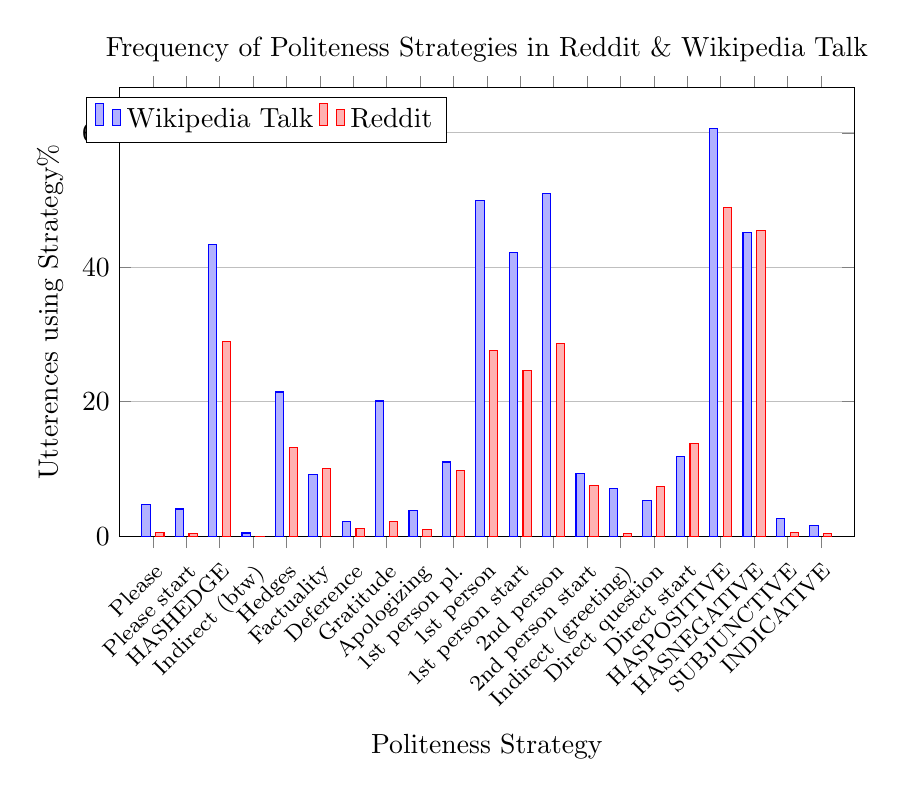
\begin{tikzpicture}
    \begin{axis}[
        ybar,
        ymin=0,
        ylabel={Utterences using Strategy\%},
        xlabel={Politeness Strategy},
        title={Frequency of Politeness Strategies in Reddit \& Wikipedia Talk},
        symbolic x coords={Please, Please start, HASHEDGE, Indirect (btw), Hedges, Factuality, Deference, Gratitude, Apologizing, 1st person pl., 1st person, 1st person start, 2nd person, 2nd person start, Indirect (greeting), Direct question, Direct start, HASPOSITIVE, HASNEGATIVE, SUBJUNCTIVE, INDICATIVE},
        xtick=data,
        ymajorgrids=true,
        enlarge x limits=0.05,
        width=0.9\textwidth,
        height=0.6\textwidth,
        legend style={at={(0.20,0.98)},anchor=north,legend columns=-1},
        xticklabel style={rotate=45,anchor=north east},
        xticklabel style={font=\footnotesize}, % Optional: Adjust font size
        bar width=3pt
    ]
    \addplot coordinates {
        (Please,4.68)(Please start,4.04)(HASHEDGE,43.42)(Indirect (btw),0.48)(Hedges,21.46)(Factuality,9.13)(Deference,2.24)(Gratitude,20.12)(Apologizing,3.87)(1st person pl.,11.04)(1st person,49.93)(1st person start,42.16)(2nd person,50.93)(2nd person start,9.32)(Indirect (greeting),7.09)(Direct question,5.34)(Direct start,11.8)(HASPOSITIVE,60.64)(HASNEGATIVE,45.17)(SUBJUNCTIVE,2.57)(INDICATIVE,1.56)
    };
    \addplot coordinates {
        (Please,0.55)(Please start,0.36)(HASHEDGE,28.93)(Indirect (btw),0.02)(Hedges,13.19)(Factuality,10.05)(Deference,1.08)(Gratitude,2.24)(Apologizing,1.02)(1st person pl.,9.73)(1st person,27.59)(1st person start,24.61)(2nd person,28.72)(2nd person start,7.58)(Indirect (greeting),0.44)(Direct question,7.35)(Direct start,13.83)(HASPOSITIVE,48.88)(HASNEGATIVE,45.53)(SUBJUNCTIVE,0.55)(INDICATIVE,0.46)
    };
    \legend{Wikipedia Talk, Reddit}
    \end{axis}
\end{tikzpicture}